\documentclass[11pt]{article}
\usepackage{cornell-notes}
\usepackage{mathtools}
\usepackage{needspace}
\usepackage{ragged2e}
\usepackage{adjustbox}
\usepackage{tikz}
\usetikzlibrary{arrows.meta,positioning}
\tcbuselibrary{most}
\geometry{letterpaper,margin=0.72in,headheight=15pt}
\setCornellCollection{Calculus Cornell Notes}
\setCornellUnitType{Chapter}
\setCornellUnitNumber{12}
\setCornellUnitTitle{Vector-Valued Functions}

\definecolor{Ink}{HTML}{17324D}
\definecolor{Teal}{HTML}{147D78}
\definecolor{Sky}{HTML}{DDEEF1}
\definecolor{Cue}{HTML}{EEF2F5}
\definecolor{Warm}{HTML}{FFF3D6}
\definecolor{Alert}{HTML}{9D3C32}
\definecolor{Green}{HTML}{276749}
\definecolor{Rule}{HTML}{AAB8C2}
\hypersetup{colorlinks=true,linkcolor=Ink,urlcolor=Teal,pdfborder={0 0 0}}
\setlength{\parindent}{0pt}
\setlength{\parskip}{4pt}
\setlist{nosep,leftmargin=*}
\titleformat{\section}{\Large\bfseries\color{Ink}}{}{0pt}{}[\color{Teal}\titlerule]
\titleformat{\subsection}{\large\bfseries\color{Teal}}{}{0pt}{}
\pagestyle{fancy}
\fancyhf{}
\fancyhead[L]{\small\color{Ink}\textsc{Cornell Notes}}
\fancyhead[R]{\small\color{Teal}\nouppercase{\leftmark}}
\fancyfoot[L]{\footnotesize\color{Ink}Active recall $\bullet$ Worked reasoning $\bullet$ Verification}
\fancyfoot[R]{\footnotesize\color{Ink}\thepage\ of \pageref*{LastPage}}
\renewcommand{\headrulewidth}{0.5pt}
\renewcommand{\footrulewidth}{0.4pt}
\newcolumntype{Y}{>{\RaggedRight\arraybackslash}X}
\newtcolorbox{orientationbox}{enhanced,breakable,colback=Sky,colframe=Teal,boxrule=0.7pt,arc=2mm,title=Chapter orientation,fonttitle=\bfseries}
\newtcolorbox{sectionsummarybox}{enhanced,breakable,colback=white,colframe=Teal,boxrule=0.6pt,arc=1.5mm,left=2mm,right=2mm,top=1mm,bottom=1mm,title=Section synthesis,fonttitle=\bfseries\color{Teal}}
\newtcolorbox{warningbox}{enhanced,breakable,colback=Warm,colframe=Alert,boxrule=0.7pt,arc=1.5mm,title=Common error audit,fonttitle=\bfseries}
\newtcolorbox{checkbox}{enhanced,breakable,colback=white,colframe=Green,boxrule=0.7pt,arc=1.5mm,title=Verification habit,fonttitle=\bfseries}
\newcommand{\cornellcuehead}{\rowcolor{Ink}\color{white}\bfseries Cue / recall prompt & \color{white}\bfseries Notes / reasoning \\\endhead}
\newcommand{\cornellcuerow}[2]{\rowcolor{Cue}#1 & #2 \\\addlinespace[3pt]}
\newcommand{\formula}[1]{\begin{tcolorbox}[colback=Sky,colframe=Teal,boxrule=0.5pt,arc=1mm,left=2mm,right=2mm,top=1mm,bottom=1mm]\centering\adjustbox{max width=0.97\linewidth}{$\displaystyle #1$}\end{tcolorbox}}

\title{Chapter 12: Vector-Valued Functions\\[2mm]\large Cornell Notes}
\author{}
\date{}
\hypersetup{pdftitle={Chapter 12: Vector-Valued Functions - Cornell Notes},pdfauthor={},pdfsubject={Calculus study notes},pdfkeywords={calculus, Cornell notes, active recall}}
\begin{document}
\maketitle
\thispagestyle{fancy}
\begin{orientationbox}
Describe curves and motion in space with vector-valued functions, then analyze derivatives, frames, arc length, and curvature. These notes follow the complete local section sequence (819--870) and emphasize definitions, governing results, strategy selection, and verifiable reasoning.
\end{orientationbox}

\section{Prerequisite map}
\begin{minipage}[t]{0.42\textwidth}
\textbf{Bring forward}
\begin{itemize}
\item Vectors
\item Parametric curves
\item Single-variable differentiation
\item Arc length
\end{itemize}
\end{minipage}\hfill
\begin{minipage}[t]{0.54\textwidth}
\textbf{Chapter flow}
\begin{center}
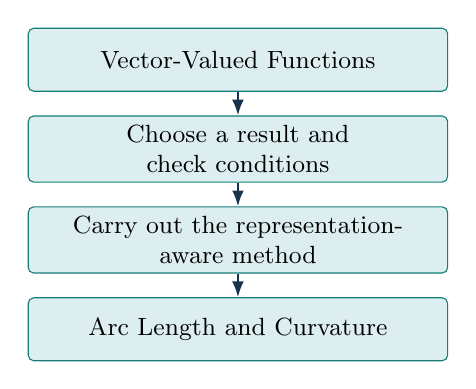
\begin{tikzpicture}[node distance=3mm, every node/.style={font=\small,align=center}, box/.style={draw=Teal,rounded corners=2pt,fill=Sky,minimum height=8mm,text width=0.42\textwidth}, arr/.style={-{Latex[length=2mm]},thick,draw=Ink}]
\node[box] (a) {Vector-Valued Functions};
\node[box,below=of a] (b) {Choose a result and check conditions};
\node[box,below=of b] (c) {Carry out the representation-aware method};
\node[box,below=of c] (d) {Arc Length and Curvature};
\draw[arr] (a)--(b); \draw[arr] (b)--(c); \draw[arr] (c)--(d);
\end{tikzpicture}
\end{center}
\end{minipage}

\section{Learning objectives}
\begin{enumerate}
\item Explain the central objects and hypotheses in 12.1 and 12.5.
\item Translate among algebraic, graphical, numerical, and verbal representations.
\item Select an appropriate formula or theorem before beginning symbolic work.
\item Carry out multi-step calculations while preserving domain, sign, orientation, and units.
\item Diagnose common errors by testing assumptions and checking the result independently.
\item Synthesize the chapter's methods into a reusable problem-solving workflow.
\end{enumerate}

\section{12.1 Vector-Valued Functions}
\begin{longtable}{C N}\cornellcuehead
\cornellcuerow{What is the governing idea in 12.1?}{A vector-valued function traces a curve by assigning a position vector to each parameter value.}
\cornellcuerow{Which result should be recalled?}{\formula{\mathbf r(t)=f(t)\mathbf i+g(t)\mathbf j+h(t)\mathbf k}}
\cornellcuerow{How should a problem be organized?}{State the parameter domain, inspect component functions, eliminate the parameter only with restrictions, and identify orientation.}
\cornellcuerow{What should be checked before accepting an answer?}{Confirm the hypotheses and domain, preserve units and orientation when relevant, and substitute or differentiate back into the defining relation.}
\end{longtable}
\begin{warningbox}The curve's geometric image does not by itself record speed, direction, or repeated traversal.\end{warningbox}
\begin{sectionsummarybox}A vector-valued function traces a curve by assigning a position vector to each parameter value. The operational habit is to state the parameter domain, inspect component functions, eliminate the parameter only with restrictions, and identify orientation.\end{sectionsummarybox}
\section{12.2 Differentiation and Integration of Vector-Valued Functions}
\begin{longtable}{C N}\cornellcuehead
\cornellcuerow{What is the governing idea in 12.2?}{Vector limits, derivatives, and integrals operate componentwise and obey vector product rules.}
\cornellcuerow{Which result should be recalled?}{\formula{\mathbf r'(t)=\langle f'(t),g'(t),h'(t)\rangle}}
\cornellcuerow{How should a problem be organized?}{Differentiate components, apply dot and cross product rules in the correct order, and use initial vectors to determine integration constants.}
\cornellcuerow{What should be checked before accepting an answer?}{Confirm the hypotheses and domain, preserve units and orientation when relevant, and substitute or differentiate back into the defining relation.}
\end{longtable}
\begin{warningbox}A vector antiderivative requires a constant vector, not one scalar constant.\end{warningbox}
\begin{sectionsummarybox}Vector limits, derivatives, and integrals operate componentwise and obey vector product rules. The operational habit is to differentiate components, apply dot and cross product rules in the correct order, and use initial vectors to determine integration constants.\end{sectionsummarybox}
\section{12.3 Velocity and Acceleration}
\begin{longtable}{C N}\cornellcuehead
\cornellcuerow{What is the governing idea in 12.3?}{Position differentiates to velocity and acceleration; speed is the magnitude of velocity.}
\cornellcuerow{Which result should be recalled?}{\formula{\mathbf v=\mathbf r',\qquad \mathbf a=\mathbf r'',\qquad \text{speed}=\|\mathbf v\|}}
\cornellcuerow{How should a problem be organized?}{Differentiate the position vector, separate vector velocity from scalar speed, and use initial conditions to reconstruct motion.}
\cornellcuerow{What should be checked before accepting an answer?}{Confirm the hypotheses and domain, preserve units and orientation when relevant, and substitute or differentiate back into the defining relation.}
\end{longtable}
\begin{warningbox}Constant speed does not imply zero acceleration because direction may change.\end{warningbox}
\begin{sectionsummarybox}Position differentiates to velocity and acceleration; speed is the magnitude of velocity. The operational habit is to differentiate the position vector, separate vector velocity from scalar speed, and use initial conditions to reconstruct motion.\end{sectionsummarybox}
\section{12.4 Tangent Vectors and Normal Vectors}
\begin{longtable}{C N}\cornellcuehead
\cornellcuerow{What is the governing idea in 12.4?}{The unit tangent gives direction of motion; the principal unit normal gives the direction in which that tangent turns.}
\cornellcuerow{Which result should be recalled?}{\formula{\mathbf T=\frac{\mathbf r'}{\|\mathbf r'\|},\qquad \mathbf N=\frac{\mathbf T'}{\|\mathbf T'\|}}}
\cornellcuerow{How should a problem be organized?}{Confirm regularity, normalize velocity, differentiate the unit tangent, and check that $\mathbf T\cdot\mathbf N=0$.}
\cornellcuerow{What should be checked before accepting an answer?}{Confirm the hypotheses and domain, preserve units and orientation when relevant, and substitute or differentiate back into the defining relation.}
\end{longtable}
\begin{warningbox}Normalizing before differentiating and after differentiating are not interchangeable operations.\end{warningbox}
\begin{sectionsummarybox}The unit tangent gives direction of motion; the principal unit normal gives the direction in which that tangent turns. The operational habit is to confirm regularity, normalize velocity, differentiate the unit tangent, and check that $\mathbf T\cdot\mathbf N=0$.\end{sectionsummarybox}
\section{12.5 Arc Length and Curvature}
\begin{longtable}{C N}\cornellcuehead
\cornellcuerow{What is the governing idea in 12.5?}{Arc length accumulates speed; curvature measures change of unit tangent per unit arc length.}
\cornellcuerow{Which result should be recalled?}{\formula{L=\int_a^b\|\mathbf r'(t)\|dt,\qquad \kappa=\frac{\|\mathbf r'\times\mathbf r''\|}{\|\mathbf r'\|^3}}}
\cornellcuerow{How should a problem be organized?}{Compute speed, integrate over the correct traversal, and choose the curvature formula that avoids unnecessary algebra.}
\cornellcuerow{What should be checked before accepting an answer?}{Confirm the hypotheses and domain, preserve units and orientation when relevant, and substitute or differentiate back into the defining relation.}
\end{longtable}
\begin{warningbox}A nonregular parameter point with $\mathbf r'=\mathbf0$ makes tangent and curvature formulas invalid.\end{warningbox}
\begin{sectionsummarybox}Arc length accumulates speed; curvature measures change of unit tangent per unit arc length. The operational habit is to compute speed, integrate over the correct traversal, and choose the curvature formula that avoids unnecessary algebra.\end{sectionsummarybox}

\section{Definitions and theorem register}
\small
\begin{longtable}{@{}>{\RaggedRight\arraybackslash}p{0.24\textwidth}>{\RaggedRight\arraybackslash}p{0.40\textwidth}>{\RaggedRight\arraybackslash}p{0.29\textwidth}@{}}
\toprule
\textbf{Topic} & \textbf{Meaning and conditions} & \textbf{Canonical form}\\
\midrule\endhead
12.1 Vector-Valued Functions & A vector-valued function traces a curve by assigning a position vector to each parameter value. & \adjustbox{max width=\linewidth}{\(\displaystyle \mathbf r(t)=f(t)\mathbf i+g(t)\mathbf j+h(t)\mathbf k\)} \\\addlinespace[2pt]
12.2 Differentiation and Integration of Vector-Valued Functions & Vector limits, derivatives, and integrals operate componentwise and obey vector product rules. & \adjustbox{max width=\linewidth}{\(\displaystyle \mathbf r'(t)=\langle f'(t),g'(t),h'(t)\rangle\)} \\\addlinespace[2pt]
12.3 Velocity and Acceleration & Position differentiates to velocity and acceleration; speed is the magnitude of velocity. & \adjustbox{max width=\linewidth}{\(\displaystyle \mathbf v=\mathbf r',\qquad \mathbf a=\mathbf r'',\qquad \text{speed}=\|\mathbf v\|\)} \\\addlinespace[2pt]
12.4 Tangent Vectors and Normal Vectors & The unit tangent gives direction of motion; the principal unit normal gives the direction in which that tangent turns. & \adjustbox{max width=\linewidth}{\(\displaystyle \mathbf T=\frac{\mathbf r'}{\|\mathbf r'\|},\qquad \mathbf N=\frac{\mathbf T'}{\|\mathbf T'\|}\)} \\\addlinespace[2pt]
12.5 Arc Length and Curvature & Arc length accumulates speed; curvature measures change of unit tangent per unit arc length. & \adjustbox{max width=\linewidth}{\(\displaystyle L=\int_a^b\|\mathbf r'(t)\|dt,\qquad \kappa=\frac{\|\mathbf r'\times\mathbf r''\|}{\|\mathbf r'\|^3}\)} \\\addlinespace[2pt]
\bottomrule
\end{longtable}
\normalsize

\section{Formula and method sheet}
\small
\begin{longtable}{@{}>{\RaggedRight\arraybackslash}p{0.08\textwidth}>{\RaggedRight\arraybackslash}p{0.48\textwidth}>{\RaggedRight\arraybackslash}p{0.37\textwidth}@{}}
\toprule
\textbf{Sec.} & \textbf{Method sequence} & \textbf{Stop-and-check trigger}\\
\midrule\endhead
12.1 & State the parameter domain, inspect component functions, eliminate the parameter only with restrictions, and identify orientation. & The curve's geometric image does not by itself record speed, direction, or repeated traversal. \\\addlinespace[2pt]
12.2 & Differentiate components, apply dot and cross product rules in the correct order, and use initial vectors to determine integration constants. & A vector antiderivative requires a constant vector, not one scalar constant. \\\addlinespace[2pt]
12.3 & Differentiate the position vector, separate vector velocity from scalar speed, and use initial conditions to reconstruct motion. & Constant speed does not imply zero acceleration because direction may change. \\\addlinespace[2pt]
12.4 & Confirm regularity, normalize velocity, differentiate the unit tangent, and check that $\mathbf T\cdot\mathbf N=0$. & Normalizing before differentiating and after differentiating are not interchangeable operations. \\\addlinespace[2pt]
12.5 & Compute speed, integrate over the correct traversal, and choose the curvature formula that avoids unnecessary algebra. & A nonregular parameter point with $\mathbf r'=\mathbf0$ makes tangent and curvature formulas invalid. \\\addlinespace[2pt]
\bottomrule
\end{longtable}
\normalsize

\section{Common errors and diagnostic checks}
\begin{warningbox}
\begin{itemize}
\item \textbf{12.1:} The curve's geometric image does not by itself record speed, direction, or repeated traversal.
\item \textbf{12.2:} A vector antiderivative requires a constant vector, not one scalar constant.
\item \textbf{12.3:} Constant speed does not imply zero acceleration because direction may change.
\item \textbf{12.4:} Normalizing before differentiating and after differentiating are not interchangeable operations.
\item \textbf{12.5:} A nonregular parameter point with $\mathbf r'=\mathbf0$ makes tangent and curvature formulas invalid.
\end{itemize}
\end{warningbox}
\begin{checkbox}
Before accepting any result: state the relevant domain; check theorem hypotheses; estimate sign and scale; preserve units and orientation; and verify by substitution, differentiation, a limiting case, or a second representation.
\end{checkbox}

\section{Chapter synthesis}
Describe curves and motion in space with vector-valued functions, then analyze derivatives, frames, arc length, and curvature. The chapter begins with \textbf{Vector-Valued Functions} and culminates in \textbf{Arc Length and Curvature}. Across the sequence, the most reliable workflow is to identify the mathematical object, choose a representation, state the governing result with its hypotheses, compute without dropping restrictions, and audit the answer against the original definition. Vector-valued calculus separates path geometry from parametrized motion: derivatives, speed, frames, and curvature are meaningful only with regularity and parameter interpretation.

\section{Self-test questions}
\begin{enumerate}
\item Explain the central distinction or object in 12.1, using both words and notation.
\item State the main formula or result from 12.2 and identify every hypothesis or restriction needed for its use.
\item Describe the problem-solving procedure for 12.3. What is the strongest independent check?
\item Compare the roles of Vector-Valued Functions and Arc Length and Curvature within this chapter.
\item Reconstruct the governing formula for 12.4 from its geometric or analytic meaning.
\item Choose one method in the chapter and explain how its output should be interpreted, including units or orientation when applicable.
\item Scenario: A student working on 12.1 produces a polished calculation but makes this error: The curve's geometric image does not by itself record speed, direction, or repeated traversal. Diagnose the earliest invalid step and repair the workflow.
\item Scenario: A solution in 12.2 quotes the displayed formula without checking conditions. Which conditions must be checked, and what could fail if they are absent?
\item Construct a concept map linking a representation, a governing result, a computation, and a verification check from this chapter.
\item Design a two-part test for mastery: one conceptual prompt and one calculation. State what evidence would count as a complete answer.
\end{enumerate}

\Needspace{8\baselineskip}
\section{Answer key}
\small
\begin{enumerate}
\item A complete response identifies A vector-valued function traces a curve by assigning a position vector to each parameter value. It should connect that meaning to \(\mathbf r(t)=f(t)\mathbf i+g(t)\mathbf j+h(t)\mathbf k\) and state the relevant domain.
\item The organizing result is \(\mathbf r'(t)=\langle f'(t),g'(t),h'(t)\rangle\). The solver must check that the quantities are defined and that the assumptions named in 12.2 hold before applying it.
\item Use this sequence: Differentiate the position vector, separate vector velocity from scalar speed, and use initial conditions to reconstruct motion. The strongest check is to return to the defining relation or differentiate/substitute the result, as appropriate.
\item Vector-Valued Functions establishes a vector-valued function traces a curve by assigning a position vector to each parameter value. Arc Length and Curvature extends the chapter to arc length accumulates speed; curvature measures change of unit tangent per unit arc length. The connection is the reuse of the same representations under a broader method.
\item The formula \(\mathbf T=\frac{\mathbf r'}{\|\mathbf r'\|},\qquad \mathbf N=\frac{\mathbf T'}{\|\mathbf T'\|}\) follows by translating the defining geometric or rate relationship into symbols; each factor records a distinct change or scale.
\item Interpretation must name what varies, with respect to what, and on which domain. A numerical value without units, sign, direction, or interval information is incomplete whenever those features are part of the modeled quantity.
\item The earliest fault is the unverified assumption described by this warning: The curve's geometric image does not by itself record speed, direction, or repeated traversal. Restart by following this procedure: State the parameter domain, inspect component functions, eliminate the parameter only with restrictions, and identify orientation.
\item The formula \(\mathbf r'(t)=\langle f'(t),g'(t),h'(t)\rangle\) is conditional, not decorative. Check domain, differentiability or integrability as relevant, boundary or orientation requirements, and nonzero denominators before drawing a conclusion.
\item One valid map is: the representation in 12.1 identifies the object; the result in 12.2 supplies a rule; the method in 12.3 carries out the computation; the check in 12.5 tests the conclusion against its definition.
\item The conceptual prompt should require explanation of a definition and its hypotheses. The calculation should require method selection rather than direct substitution. Full evidence includes setup, justified transformations, a result, and an independent check.
\end{enumerate}
\normalsize

\section{Key-term recap}
\small
\begin{longtable}{@{}>{\RaggedRight\arraybackslash}p{0.29\textwidth}>{\RaggedRight\arraybackslash}p{0.64\textwidth}@{}}
\toprule
\textbf{Term} & \textbf{Working meaning}\\
\midrule\endhead
Vector-Valued Functions & A vector-valued function traces a curve by assigning a position vector to each parameter value. \\\addlinespace[2pt]
Differentiation and Integration of Vector-Valued Functions & Vector limits, derivatives, and integrals operate componentwise and obey vector product rules. \\\addlinespace[2pt]
Velocity and Acceleration & Position differentiates to velocity and acceleration; speed is the magnitude of velocity. \\\addlinespace[2pt]
Tangent Vectors and Normal Vectors & The unit tangent gives direction of motion; the principal unit normal gives the direction in which that tangent turns. \\\addlinespace[2pt]
Arc Length and Curvature & Arc length accumulates speed; curvature measures change of unit tangent per unit arc length. \\\addlinespace[2pt]
\bottomrule
\end{longtable}
\normalsize

\enlargethispage{4\baselineskip}
\begin{tcolorbox}[title=One-sentence takeaway,fonttitle=\bfseries,colback=Ink,colframe=Ink,coltext=white,coltitle=white,arc=2mm,boxrule=0pt]
\centering\bfseries Vector-valued calculus separates path geometry from parametrized motion: derivatives, speed, frames, and curvature are meaningful only with regularity and parameter interpretation.
\end{tcolorbox}
\end{document}
